%%%%%%%%%%%%%%%%%%%%%%% file template.tex %%%%%%%%%%%%%%%%%%%%%%%%%
%
% This is a general template file for the LaTeX package SVJour3
% for Springer journals.          Springer Heidelberg 2010/09/16
%
% Copy it to a new file with a new name and use it as the basis
% for your article. Delete % signs as needed.
%
% This template includes a few options for different layouts and
% content for various journals. Please consult a previous issue of
% your journal as needed.
%
%%%%%%%%%%%%%%%%%%%%%%%%%%%%%%%%%%%%%%%%%%%%%%%%%%%%%%%%%%%%%%%%%%%
%
% First comes an example EPS file -- just ignore it and
% proceed on the \documentclass line
% your LaTeX will extract the file if required
\begin{filecontents*}{example.eps}
%!PS-Adobe-3.0 EPSF-3.0
%%BoundingBox: 19 19 221 221
%%CreationDate: Mon Sep 29 1997
%%Creator: programmed by hand (JK)
%%EndComments
gsave
newpath
  20 20 moveto
  20 220 lineto
  220 220 lineto
  220 20 lineto
closepath
2 setlinewidth
gsave
  .4 setgray fill
grestore
stroke
grestore
\end{filecontents*}
%
\RequirePackage{fix-cm}
%
%\documentclass{svjour3}                     % onecolumn (standard format)
%\documentclass[smallcondensed]{svjour3}     % onecolumn (ditto)
\documentclass[smallextended]{svjour3}       % onecolumn (second format)
%\documentclass[twocolumn]{svjour3}          % twocolumn
%
\smartqed  % flush right qed marks, e.g. at end of proof
%
\usepackage{graphicx}
\usepackage{cite}
\usepackage{amsmath}
\usepackage{mathtools}
\usepackage{multirow}
%\usepackage{algpseudocode}
%\usepackage[none]{hyphenat}
\usepackage{algorithm}
\usepackage{hyperref}
\usepackage[noend]{algorithmic}
%\usepackage[]{algorithm2e}
\usepackage[normalem]{ulem}
 \useunder{\uline}{\ul}{}


\newcommand{\DCN}{{\sc dcn}}
\newcommand{\DE}{{\sc de}}
\newcommand{\DEEDM}{{\sc de-edm}}
\newcommand{\EAS}{{\sc ea}s}
\newcommand{\EA}{{\sc ea}}
\newcommand{\RMDDC}{{\sc rmddc}}
\newcommand{\CEC}{{\sc cec}}
%
%%
%\usepackage{natbib}
%
% \usepackage{mathptmx}      % use Times fonts if available on your TeX system
%
% insert here the call for the packages your document requires
%\usepackage{latexsym}
% etc.
%
% please place your own definitions here and don't use \def but
% \newcommand{}{}
%
% Insert the name of "your journal" with
% \journalname{myjournal}
%
\begin{document}

\title{Differential Evolution with Enhanced Diversity Maintenance%\thanks{Grants or other notes
%about the article that should go on the front page should be
%placed here. General acknowledgments should be placed at the end of the article.}
}
%\subtitle{Do you have a subtitle?\\ If so, write it here}

%\titlerunning{Short form of title}        % if too long for running head

\author{Joel Chac\'on Castillo        \and
        Carlos Segura %etc.
}

%\authorrunning{Short form of author list} % if too long for running head

\institute{Joel Chac\'on Castillo \at
							Centro de Investigaci\'{o}n en Matemáticas, Guanajuato, Mexico\\
              \email{joel.chacon@cimat.mx}           %  \\
%             \emph{Present address:} of F. Author  %  if needed
           \and
					Carlos Segura \at
					Centro de Investigaci\'{o}n en Matemáticas, Guanajuato, Mexico\\
					\email{carlos.segura@cimat.mx}
}

\date{Received: date / Accepted: date}
% The correct dates will be entered by the editor


\maketitle

\begin{abstract}
Differential Evolution (\DE{}) is a popular population-based meta-heuristic that has been successfully used in complex 
optimization problems.
%
Premature convergence is one of the most important drawbacks that affects its performance.
%
%In combinatorial optimization, an alternative to alleviate premature convergence in memetic algorithms has been to 
%explicitly control the diversity of the population.
%
%However, this choice it is not usually applied in continuous optimization.
%
In this paper is proposed a replacement strategy that with an elite population aims to preserve diversity explicitly.
%Principally, in this paper is proposed a replacement strategy and an elite population, which are designed to preserve diversity.
%
The proposal is extended and integrated with \DE{} to generate the \DE{} with Enhanced Diversity Maintenance (\DEEDM{}).
%
The main novelty is the use of a dynamic balance between exploration and exploitation to adapt the proposal to the 
requirements of the different optimization stages.
%
%Also, our proposal applies several popular techniques, such as an elite external population.
%
Experimental validation is carried out with several benchmark tests proposed in competitions of the well-known IEEE Congress on 
Evolutionary Computation.
%
Top-rank algorithms of each competition are used to illustrate the usefulness of the proposal.
%
The new method avoids premature convergence and significantly improves further the results obtained by state-of-the-art algorithms.

\keywords{Diversity \and Differential Evolution \and Premature Convergence}
% \PACS{PACS code1 \and PACS code2 \and more}
% \subclass{MSC code1 \and MSC code2 \and more}
\end{abstract}

%%%\begin{abstract}
%%%Differential Evolution (\DE{}) is a popular population-based metaheuristic that has been successfully used in complex 
%%%optimization problems.
%%%%
%%%Premature convergence is one of the most important drawbacks that affects its performance.
%%%%
%%%In combinatorial optimization, an alternative to alleviate premature convergence in memetic algorithms has been to 
%%%explicitly control the diversity of the population.
%%%%
%%%However, this choice it is not usually applied in continuous optimization.
%%%%
%%%In this paper, a recently proposed replacement strategy to preserve diversity is extended and integrated with \DE{}
%%%to generate the \DE{} with Enhanced Diversity Maintenance (\DEEDM{}).
%%%%
%%%The main novelty is the use of a dynamic balance between exploration and exploitation to adapt the proposal to the 
%%%requirements of the different optimization stages.
%%%%
%%%Experimental validation is carried out with several benchmark tests proposed in competitions of the well-known IEEE Congress on 
%%%Evolutionary Computation.
%%%%
%%%Top-rank algorithms of each competition are used to illustrate the usefulness of the proposal.
%%%%
%%%The new method avoids premature convergence and significantly improves further the results obtained by state-of-the-art algorithms.
%%%
%%%\keywords{Diversity \and Differential Evolution \and Premature Convergence}
%%%% \PACS{PACS code1 \and PACS code2 \and more}
%%%% \subclass{MSC code1 \and MSC code2 \and more}
%%%\end{abstract}



\section{Introduction}
\label{sec:Introduction}
Los Algoritmos Evolutivos (Evolutionary Algorithms \EA{}) son considerados como uno de los enfoques con mayor aficacia para resolver distintas categorías de optimización.
%
Particularmente, se han aplicado en problemas tanto de dominio continuo \cite{glover2005handbook} como de dominio discreto.
%
Especialmente, los \EAS{} son aplicados para resolver problemas complejos cuyo enfoque determinístico es complicado o imposible~\cite{chakraborty2008advances}.
% 
Además, diversas variantes se han utilizado y aplicado en muchos campos, como es en ciencia, economía e ingeniería.
%
%
Actualmente, los \EAS{} son plenamente conocidos como metaheurísticas \cite{glover2005handbook}.
%
A pesar del éxito que tienen los \EAS{}, existe una dificultad en su adaptación o configuración ante nuevos problemas.
%
Una dificultad popular en el diseño de un \EA{} es obtener un balanceo propio entre exploración y explotación \cite{herrera1996adaptation}.
%
Sin embargo, no siempre son comprendidas las implicaciones al mantener un grado de diversidad en este balanceo y como son promovidas las exploración y explotación \cite{Crepinsek:13}.
%
Desde su inicio los \EAS{} han presentado problemas de convergencia siendo como una desventaja importante\cite{Crepinsek:13}.
%
La convergencia prematura es originada cuando todos los miembros de la población están ubicados en una parte reducida del espacio de búsqueda, esta región es distinta a la región óptima y además los componentes seleccionados no son suficientes para escapar de esta región.
%
Basado en esto se han desarrollado varias estrategias para aliviar este problems.
%
Además en através de varios estudios se ha revelado que mantener una populación diversa en un requisito previo para evitar la convergencia prematura~\cite{Crepinsek:13}.
%
Sin embargo, si la población es muy diversa, entonces un grado adecuado de explotación podría ser prevenido, resultando en un convergencia lenta y por lo tanto soluciones de baja calidad.
%
Por esta razón, Mahfoud~\cite{dasgupta2013evolutionary} utilizó el concepto de diversidad util, con cual se refiere a la cantidad de diversidad que resulta en soluciones de alta calidad.
%
En la literatura existen distintas forma para aliviar el problema de convergencia prematura~\cite{pandey2014comparative}.
%
En los 90s, la mayoría de estrategias para aliviar la convergencia prematura se centraron en modificar el esquema de selección de padres.
%
La principal razón es que en esa época la mayoría de esquemas eran generacionales, por lo tanto la presión de selección estaba definida principalmente en la selección de padres.
%
Sin embargo, se descubrió que tratando de aliviar la convergencia prematura donde únicamente sea considerada la selección de padres no fue suficiente~\cite{blickle1996comparison}.
%
Posteriormente, la una gran cantidad de \EAS{} incorporaron una fase de reemplazo que abandonaron al menos parcialmente a los métodos generacionales iniciales.
%
Basado en esto muchos autores descubrieron la posibilidad de incorporar métodos para aliviar el problema de convergencia prematura~\cite{Crepinsek:13}.
%
Es importante considerar que aún cuando los métodos de reemplazamiento generacionales~\cite{de2006evolutionary} fueron suficientemente populares, algunos autores ya habían tomado en cuenta esta estrategia~\cite{mahfoud1992crowding}.
%
Sin embargo, con la efectividad de elitismo y otras estrategias de reemplazo, el número de esquemas que adoptaron estos principios crecieron de forma considerable~\cite{lozano2008replacement}.
%

Un aspecto importante de la convergencia prematura es que depende completamente de la cantidad de tiempo y/o generaciones asignados a las ejecuciones del \EA{}, es decir el criterio de paro.
%
En su lugar, un \EA{} debería ser ejecutado para resolver un problema dado por un tiempo definido y éste debería proporcionar soluciones prometedoras.
%
A pesar de esto, es sorprendente que la mayoría de métodos que se han propuesto para aliviar la desventaja de la convergencia prematura no consideran el criterio de paro el cual es asignado por el usuario para alterar su comportamiento interno.
%
Esto significa que, dependiendo en el criterio de paro, distintas parametrizaciones podrían ser requeridas.
%
Como resultado, para criterio de paro distinto, el usuario debería estudiar el efecto de distintos parámetros.
%
Un ejemplo popular de esto es \textit{El Torneo de Selección Restringida (TSR)}~\cite{Crepinsek:13}, este método retrasa la convergencia de los \EAS{}.
%
Específicamente, este método incorpora un parámetro que puede ser utilizado para alterar el balanceo entre exploración e intensificación.
%
Sin embargo, la pérdida de diversidad y posteriormente el balanceo entre exploración e intensificación no dependen únicamente en este parámetro, por lo tanto distintos valores deberían ser utilizados para cada problema y además para cada criterio de paro.
%
El principio básico de las técnicas para la preservación de la diversidad y que afectan a la fase de reemplazo se basa en que el efecto de diversificar a los sobrevivientes inducide un mayor grado de exploración.
%
Esto se debe a varios aspectos importantes, principalmente una población grande mantiene varias regiones del espacio de búsqueda.
%
Además los operadores de cruce tienden a se más explorativos cuando están involucrados individuos distantes \cite{eiben1998evolutionary}.


Entre las distintas categorías de \EAS{}, Evolución Diferencial (Differential Evolution - \DE{}) es una de las estrategias más efectivas para lidiar con problemas de optimización contínua~\cite{storn1997differential}.
%
De hecho, esta categoría de algoritmos han sido los ganadores en varias competencias de optimización~\cite{das2011differential}.
%
Similarmente a otros \EAS{}. \DE{} está inspirado en el proceso de evolución natural, y además involucra la aplicaciónde mutación, recombinación y selección.
%
La principal característica de \DE{} es que éste considera las diferencias de los vectores que están presentes en la población con el motivo de explorar el espacio de búsqueda.
%
En este sentido \DE{} es similar a los optimizadores \textit{Nelder-Mead}~\cite{nelder1965simplex}  y a la \textit{Búsqueda Aleatoria Controlada (BAC)} \cite{price1983global}.
%
A pesar de la efectividad de \DE{}, existen varias debilidades que han sido detectadas y resueltas de forma parcial que por lo tanto a generado extensiones a la variante estándar de \DE{}~\cite{das2011differential}.
%
Algunos de los problemas más conocidos es la sensibilidad de la parametrización~\cite{zhang2009jade}, la apariencia de estancamiento debido a las capacidades de exploración reducidas~\cite{sa2008exploration,lampinen2000stagnation} y la convergencia prematura~\cite{zaharie2003control}.
%
Desde la aparición de \DE{}, varias críticas se hicieron debido a su falta de capacidad para mantener un grado de diversidad suficiente dado a la elevada presión de selección~\cite{sa2008exploration}.
%
Por lo tanto, se han generado varias extensiones de \DE{} para aliviar la convergencia prematura, como la adaptiación de parámetros~\cite{zaharie2003control}, auto-adaptación de la diversidad en la población~\cite{yang2015differential} y estrategias de selección con una menor presión de selección~\cite{sa2008exploration}.
%
Algúnos de los últimos estudios en el diseño metaheurísticas poblacionales~\cite{Crepinsek:13} mostraron que controlando explícitamente la diversidad es particularmente útil para obtener un propio balanceo entre el grado de exploración y de intensificación.
%
Nuestra hipótesis es que introduciendo un mecanismo para la preservación de la diversidad results en un balanceo adecuado entre exploración e intensidifación, que a su vez propociona soluciones de alta calidad en ejecuciones a largo plazo.

Principalmente en este capítulo se explican dos propuestas, primeramente \DE{} con Mantenimiento de Diversidad Mejorado ( \DE with Enhanced Diversity Maintenance\DEEDM{}), el cual integra un principio similar en \DE{} y el operador Dinámico basado en el Cruce Binario Simulado ( Dynamic Simulated Binary Crossover \DSBX{}).

Our novel proposal, which is called \DE{} with Enhanced Diversity Maintenance (\DEEDM{}), integrates a similar principle into \DE{}.
%
El resto de este capítulo está organizado de la siguiente forma.


\section{Literature Review}
\label{sec:Literature}



\section{Performance in IEEE CEC Contests}
\label{sec:trends}
In recent years, several contests have been organized at the \textsc{ieee cec} to facilitate comparisons among optimizers.
%
Such contests define set of optimization functions with different features and complexities, so analyzing the results
through the years offers insights about which are the principles and algorithms that offer more advantages.
%
This section is devoted to summarize the methods and ideas with more contributions, focusing the efforts
on \DE{} variants with the aim of detecting design tendencies on the \DE{} field. 

In \CEC{} 2005 competition on real parameter optimization~\cite{CEC2005}, classical \DE{} attained the second rank and 
the self-adaptive \DE{} variant called SaDE obtained the third rank in 10 dimensions.
%
However, they performed poorly with more than 30 dimensions.
%
Subsequently, in the 2008 competition on large scale global optimization~\cite{CEC2008}, a self-adaptive \DE{} (jDEdynNP-F) 
reached the third place, confirming the importance of parameter adaptation.
%
In fact, in other kinds of competitions such as in the 2006 constrained optimization, the benefits of adaptation 
was also shown, where SaDE obtained the third place.
%
In subsequent competition in large-scale optimization (\CEC{} 2010), \DE{} variants did not reach the top rank.
%
This, together with the fact that the performance of several \DE{} variants performed properly only in low-dimensionality, 
is an indicator of the weaknesses of \DE{} in large scale problems.
%
In fact, some of the reasons of the curse of dimensionality were analyzed in~\cite{segura2015improving}.
%
Thus, it is known that there is room for improvement in terms of scalability, although dealing with large-scale optimization is out of 
the scope of this paper.

In \CEC{} 2011 competition with real world optimization problems~\cite{CEC2011}, hybrid algorithms including \DE{} have performed
properly.
%
For instance, the second place was obtained by the hybrid \DE{} called DE-$\Lambda_{CR}$.
%
Again a Self-adaptive Multi-Operator \DE{} (SAMODE) performed properly and obtained the third place.

In recent years, adaptive variants have also stood out.
%
However, the complexity of the best schemes have increased considerably.
%
In the 2014 competition on real parameter optimization~\cite{CEC2014}, the first place was reached by the Linear Population Size 
Reduction Success-History Based Adaptive \DE{} (L-SHADE).
%
Similarly to other adaptive variants, this proposal adapts the internal parameters of \DE{} and the success-history based variants
are currently very well-known strategies.
%
In order to get a better degree between exploration and exploitation it dynamically reduces the population size.
%
In the 2015 competition based on learning~\cite{CEC2015}, a variant of the previous approach obtained the first place.
%
Additionally, two \DE{} variants with parameter adaptation attained the second and third place.

In this paper, experimental validation is focused on the \CEC{} 2016 and \CEC{} 2017 competitions in real parameter optimization.
%
In the case of 2016~\cite{CEC2015}, the first place was reached with the United Multi-Operator Evolutionary Algorithm (UMOEAs-II).
%
This approach is not a \DE{} scheme but some of the \DE{} operators are taken into account.
%
The second place was reached by Ensemble Sinusoidal Differential Covariance Matrix Adaptation with Euclidean Neighborhood (L-SHADE-EpSin) 
and the third place was attained by the Improved L-SHADE (iL-SHADE).
%
Note that the two last ones were again variants of SHADE.
%
In fact, variants of SHADE have also excelled in the learning-based competitions~\cite{CEC2016_learn}.

In the \CEC{} 2017 case~\cite{CEC2017}, the first place was obtained by the Effective Butterfly Optimizer with Covariance 
Matrix Adapted Retreat Phase (EBOwithCMAR), which is not a \DE{} variant.
%
EBOwithCMAR is an extension of UMOEAs-II.
%
The second place was reached by jSO, which is an improvement of iL-SHADE.
%
Finally, the L-SHADE-EpSin, again a variant of SHADE, attained the third place.

Attending to the features of the different approaches, the following trend is detected:

\begin{itemize}
	\item Typically, the parameters are altered during the run with the aim of adapting the optimizer to the requirements of the different optimization stages. 
	\item In some of the last algorithms, the adaptation considers the stopping criterion and elapsed generations to bias the decisions taken the optimizer.
	For instance, some proposals decrease the population size and in other cases the \DE{} are modified to intensify further in last stages.
	\item The overall complexity of the winners have increased significantly. Particularly, several variants include modifications to perform promising
	movements with a higher probability, for instance by including the principles of the Covariance Matrix Adaptation scheme.
\end{itemize}

Our proposal takes the previous conclusions into consideration.
%
However, our hypothesis is that for long-term executions simpler variants with explicit control of diversity are enough to excel and 
that some of the proposed modifications might be counter-productive.
%
For instance, it is known that the parameter adaptation might provoke some improper movements that might affect performance in the
long term~\cite{montgomery2010analysis}.
%
Note that by controlling the diversity, the degree between exploration and exploitation can be properly altered automatically.
%
As a result, parameter adaptation or modifications to alter the probability of different movements are not included in our proposal.
%
We consider that some of these modification might be beneficial but they should be included carefully.


%In the competitions of the last years SHADE's family algorithms seems to be more participatory, however based in that the ability exploration of DE is highly affected by the population size, usually the search is complemented with a Covariance Matrix Adaptation variant as is showed in the UMOEAs-II and L-SHADE-EpSin algorithms.
%
%It is also interesting to note that the variants of DE continued to secure front ranks in the subsequent CEC competitions like CEC 2006 competition on constrained real parameter optimization (first rank), CEC 2007 competition on multi-objective optimization (second rank), CEC 2008 competition on large scale global optimization (third rank), CEC 2009 competition on multi-objective optimization (first rank was taken by a DE-based algorithm MOEA/D for unconstrained problems), and CEC 2009 competition on evolutionary computation in dynamic and uncertain environments (first rank).
%




\section{Proposal}
\label{sec:Proposal}
Our proposal is motivated by two main works in the area of control of diversity in EAs.
%
The first one is the empirical study developed by Montgomery et al~\cite{montgomery2012simple},
which presents several empirical analyses that confirm issues related to premature convergence in \DE{}.
%
The second work, by Segura et al.~\cite{segura2016novel}, provides significant improvements in the combinatorial optimization field
by developing a novel replacement strategy called \textit{The Replacement with Multi-objective based Dynamic Diversity Control} (\RMDDC{}) 
that relates the control of diversity with the stopping criterion and elapsed generations.
%
Important benefits were attained by methods including \RMDDC{}, so given the conclusions of these previous works, the proposal of this paper is a 
novel \DE{} variant that includes an explicit mechanism that follows some of the principles of \RMDDC{}.
%
This novel optimizer is called \textit{Differential Evolution with Enhanced Diversity Maintenance} (\DEEDM{}) and its source
code is freely available~\footnote{The code in C++ can be downloaded in the next link \url{https://github.com/joelchaconcastillo/Diversity\_DE\_Research.git}}.

The core of \DEEDM{} (see Algorithm~\ref{alg:DEEDM}) is quite similar to the standard \DE{}.
%
In fact the way of creating new trial solutions is not modified at all (lines 5 and 6).
%
The novelty is the incorporation of an elite population ($E$) and a novel diversity-based replacement strategy.
%
In order to select the members of the elite population, the original greedy replacement of \DE{} is used (line 7).
%
On the other way, the replacement strategy (line 8) follows the same principle that guided the 
design of \RMDDC{}, i.e. individuals that contribute too little to diversity should not be accepted as members of the next generation.
%
In this way, the greedy selection strategy of \DE{} is not used to maintain the parent population ($X$).
%
In order to establish the minimum acceptable diversity contribution to be selected, the stopping criterion and elapsed
generations are taken into account.
%
One of the main weaknesses of \RMDDC{} is that its convergence is highly delayed.
%
Thus, in order to promote a faster convergence than in \RMDDC{} two modifications are performed.
%
First, no concepts of the multi-objective field are applied, instead a more greedy selection is taken into account.
%
Second, the elite population is also considered as an input of the replacement strategy.

\begin{algorithm}[t]
\algsetup{linenosize=\tiny}
  \scriptsize
	\caption{General scheme of DE-EDM} 
	\begin{algorithmic}[1]
	\STATE Randomly initialize the population of $NP$ individuals, where each one is uniformly distributed.
	\STATE $G=0$
	\WHILE{ stopping criterion is not satisfied}
	   \FOR{ $i=1$ to $NP$} 
		\STATE Mutation: Generate the donor vector ($V_{i,G}$) according Eq. (\ref{eqn:mutation}).
		\STATE Crossover: Recombine the mutate vector ($U_{i,G}$) according Eq. (\ref{eqn:crossover}).
		\STATE Selection: Update the elite vector ($E_{i,G}$ instead of $X_{i,G}$) according Eq. (\ref{eqn:selection}).
		\STATE Replacement: Select the target vectors ($X_{i,G+1}$) according to Algorithm \ref{alg:Replacement} .
	   \ENDFOR
	   \STATE $G=G+1$
	\ENDWHILE
\end{algorithmic}
    \label{alg:DEEDM}
\end{algorithm}

%\DEEDM{} alters the replacement strategy of \DE{} with the aim of controlling the 
%balance between exploration and exploitation by extending \RMDDC{}.
%
%The principles of the \RMDDC{} are as follows.
%
%It considers the maximization of the diversity contribution of each individual as an explicit objective.
%
%Then, the notion of Pareto dominance is used to select the survivors.
%
%It uses a dynamic threshold to prevent the selection of individuals with low contribution to diversity.
%
%
%Thus, executions of several days were required to attain high-quality solutions in many of the tested problems.
%
%As a result our proposal incorporates two extensions to alleviate such a drawback.
%
%This modification considers the inclusion of an elite population, which records the individuals with the best fitness.
%

Our replacement strategy (see Algorithm \ref{alg:Replacement}) operates as follows.
%
It receives as input the parent population (target vectors), the offspring population (trial vectors), and the elite population.
%
In each generation it must select the $NP$ vectors of the next parent population.
%
First, it calculates the desired minimum distance $D_t$ given the current number of elapsed function evaluations (line 2).
%
Then, it joins the three populations in a set of current members (line 3).
%
The current members set contains vectors that might be selected to survive.
%
Then, the set of survivors and penalized individuals are initialized to the empty set (line 4).
%
In order to select the $NP$ survivors (next parent population) an iterative process is repeated (lines 5 - 13).
%
In each step the best individual in the \textit{Current set}, i.e. the one with best objective function is selected
to survive, i.e. it is moved to the \textit{Survivor set} (line 6 - 8).
%
Then, individuals in the \textit{Current set} with a distance metric lower than $D_t$ are transferred to the \textit{Penalized set} (line 9).
%
%%The way to calculate the distance between two individuals is by a using a normalized Euclidean distance (Eq.~\ref{eqn:distance}).
The way to calculate the distance between two individuals is by using the normalized Euclidean distance decribed in the equation~\ref{eqn:distance}, where $D$ is the dimension of the problem, and $a_d, b_d$ are the minimum and maximum bounds of each dimension ($d$).
%
%
In cases where the \textit{Current set} is empty previous to the selection of $NP$ individuals, the \textit{Survivor set} is filled by selecting in each step 
the individual in $Penalized$ with the largest distance to the closest individual in the \textit{Survivor set}.

\begin{equation}\label{eqn:distance}
distance ( x_{i}, x_j ) = \frac{\sqrt{ \sum_{d=1}^D \left ( \frac{x_{i}^d - x_j^d}{b_d - a_d} \right )^2  }} {\sqrt{D}}
\end{equation}


\begin{algorithm}[t]
\algsetup{linenosize=\tiny}
  \scriptsize
	\caption{Replacement Phase} \label{alg:Replacement}
	\begin{algorithmic}[1]
	\STATE Input: $Population$ ($target$ $vectors$), $Offspring$ ($trial$ $vectors$), and $Elite$
	\STATE Update $D_t = D_I - D_I *(nfes/(0.95*max\_nfes)) $ 
	\STATE $Current = Population \cup Offspring \cup Elite$.
	\STATE $Survivors = Penalized = \emptyset$.
	\WHILE{ $|Survivors| < NP$ And $|Current| > 0$ }
	   \STATE $Selected$ = Select the best individual of $Current$.
		 \STATE Remove $Selected$ from $Current$.
	   \STATE Copy $Selected$ to $Survivors$.
	   \STATE Find the individuals from $Current$ with a distance to $Selected$ lower than $D_t$ and move them to $Penalized$. Normalized distance is considered (Eq. \ref{eqn:distance}).
	\ENDWHILE
	\WHILE{ $|Survivors| < NP$ }
	   \STATE $Selected$ = Select the individual from $Penalized$ with the largest distance to the closest individual in $Survivors$.
		 \STATE Remove $Selected$ from $Penalized$.
	   \STATE Copy $Selected$ to $Survivors$.
	\ENDWHILE
  \RETURN $Survivors$
\end{algorithmic}
\end{algorithm}


In order to complete the description is important to specify the way to calculate $D_t$ and the methodology to update the 
elite individuals.
%
All the remaining steps are maintained as in the classic \DE{} variant.
%
The value of $D_t$ is used to alter the degree between exploration and explotation so it should depend on the optimization stage.
%
Specifically, this value should be reduced as the stopping criterion is reached with the aim of promoting explotation.
%
In our scheme, an initial value for $D_t$ ($D_I$) must be set.
%
Then, similarly than in~\cite{segura2016novel}, a linear reduction of $D_t$ is performed by taking into account the elepased function evaluations and stopping criterion.
%
Particularly, in this work, the stopping criterion is set by function evaluations (\textit{nfes}).
%
The reduction is calculated in such way that by the $95\%$ of maximum number of evaluations the resulting $D_t$ value is $0$.
%
Therefore, in the remaining $5\%$ diversity is not considered at all.
%
Thus, if $max\_nfes$ is the maximum number of evaluations and $nfes$ is the elapsed number of evaluations, $D_t$ can be calculated as $D_t=D_I - D_I *(nfes/(0.95*max\_nfes))$.
%
%The reduction of this parameter is based in a linear reduction, as is indicated in .
%
%They indicated that a linear decrement generally provides the most stable results.
%%
%%We consider a linear model reduction based in empirical studies of similar works \cite{segura2016novel}, where they indicated that a linear decrement generally provides the most stable results.
%%%

%Principally, the replacement phase considers a defined radius ($D_t$), which for simplicity is considered through the normalized euclidean distance (Eq. \ref{eqn:distance}), however other distances could be implemented (e.g. mahalanobis distance).
%
%It is important to mention that the normalized distance is needed, thus each dimension is equally important, also this simplifies the setting of the $D_I$ parameter, since that the maximum distance is the unity, which is a fraction of the main space diagonal.


The initial distance ($D_I$) heavily affects the performance of \DEEDM{}.
%
If this parameter is fixed large enough, then at the first optimization stages the algorithm aims to maximize the diversity of the population, 
so a proper exploration is performed which is very important in some kinds of problems such as highly multimodal and deceptive ones.
%
Thus, the effect of premature convergence might be alleviated.
%
A too large $D_I$ might induce too much exploration so a proper exploitation phase is not performed.
%
In the opposite case, a too low $D_I$ might avoid the exploration phase, so avoiding local optima is more difficult.
%
Depending on the kind of fitness landscape and stopping criterion, the optimal $D_I$ might vary.
%
For instance, deceptive and highly multi-modal problems usually require larger values than unimodal problems.
%
However, in our proposal, $D_I$ is not adapted to each problem, instead an experimental study to check the robustness
of different $D_I$ value is attached in the experimental validation section. 
%
%It is interesting to take into account that our proposal could be translated to the multi-modal fashion just setting a final distance factor, which should be strictly positive, however this trend is not considered in this work.
%
%Therefore, when the initial distance factor is setted several factors should be taken into account.
%
%One of them is the maximum number of evaluations, when the problem is setted with few number of evaluations, the initial distance factor should be low, since the exploitation should be promoted.
%
%On the other hand, when the problem is configured with a large number of evaluations, then the initial distance factor should be higher.
%
%Also, the number of vectors (population size) should be considered, since that they are directly related with the diversity.
%
%Although our proposal should take into account the previously details, there exist an usual range where the results are enough stable, it is showed in the empirical analyzes.
%
%Our proposal provides several advantages in contrast of the standard DE and some of the state-of-the-art algorithms, perhaps the most important is that it is not over-parameterized.
%
%Although several top-rank algorithms present good enough results, usually these algorithms need a tuning phase to fit the parameters, therefore in real application it could be infeasible.

%
Similarly that the standard \DE{}, in \DEEDM{} the crossover probability ($CR$) and the mutation factor ($F$) must be set.
%
The first one is perhaps the most important for the performance according to several studies developed by Montgomery 
et al. \cite{montgomery2010analysis}.
%
These authors empirically proved that extremes $CR$ values leads to vastly different search behaviors.
%
They explained that low $CR$ values result in a search that is aligned with a small number of search space axes and
induce small displacements.
%
This provokes a gradual and slow convergence that in some scenarios might result in a robust behavior.
%
Additionally, high $CR$ values might generate quality solutions with a lower probability.
%
However, these transformations provoke large displacements that could improve significantly the solutions.
%
According to this, we employ both high and low $CR$ values as it is showed in Eq. \ref{eqn:cr}.

\begin{equation} \label{eqn:cr}
CR = 
\begin{cases}
     Normal(0.2, 0.1),& \text{if} \quad rand[0,1] \leq 0.5  \\
     Normal(0.9, 0.1),              & \text{otherwise}
\end{cases}
\end{equation}

Following the principles of several SHADE variants~\cite{awad2016ensemble, brest2016shade}, the function evaluations are considered in the random generation of the mutation factor $F$.
%
Particularly, each $F$ is sampled through a Cauchy distribution (Eq. \ref{eqn:cauchy}).
\begin{equation}\label{eqn:cauchy}
 Cauchy(0.5, 0.5*nfes/max\_nfes)
\end{equation}
%
Therefore, at the first optimization stages, F values near to $0.5$ are generated.
%
Then, as the execution advances, the density function suffers a gradual transformation and the variance is increased, meaning
that values outside the interval $[0.0, 1.0]$ are generated with a higher probability.
%
In the cases when values larger than $1.0$ are generated, the value $1.0$ is used.
%
In the case of generating a negative value, the $F$ is resampled.
%
One of the effects of this approach is to increase the probability of generating large $F$-values as the execution progresses
with the aim of avoiding a fast convergence.


% thus the shape of the distribution increases with the function evaluations and therefore are generated more extreme values at the end of execution, this aims avoid stagnation in different stages of the algorithm.
%


%Thus, briefly our proposal is based in several ideas of the mentioned works, and are listed as follows:
%\begin{itemize}
%\item Is considered a threshold to control explicitly the convergence of the solutions.
%\item This threshold decreases over the algorithm's run.
%\item The selection operator is relaxed in the sense that it does not provokes premature convergence, this is attained considering an elite population. 
%\end{itemize}



\section{Experimental Study}
\label{sec:Experimental}
In this section the experimental validation is presented.
%
Specifically, we show that by explicitly controlling the diversity in DE, results of state-of-the-art algorithms
are improved further.
%
Particularly, the benchmarks of \CEC{} 2016 and \CEC{} 2017 are considered.
%
Each one of them is composed of thirty different problems.
%
The state-of-the-art is composed by the algorithms that attained the first places of each year competition.
%
Thus, the algorithms considered from the \CEC{} 2016 are UMOEAs-II \cite{elsayed2016testing} and L-SHADE-EpSin \cite{awad2016ensemble} that achieved 
the first and second place respectively.
%
Similarly, the top algorithms from \CEC{} 2017 are EBOwithCMAR \cite{kumar2017improving} and jSO \cite{brest2017single}.
%
It is interesting to remark that EBOwithCMAR is considered as an improvement of the UMOEAs-II.
%
Additionally, jSO and L-SHADE-EpSin belong to the SHADE's family.
%
All these algorithms are tested with both benchmarks as it is suggested by \cite{molina2017analysis}.

Given that all of them are stochastic algorithms, each execution was repeated 51 times with different seeds.
%
In every case, the stopping criterion was set to $25,000,000$ functions evaluations.
%
We performed our evaluation following the guidelines of \CEC{} benchmark competitions.
%
Thus, if the gap between the values of the best solution found and the optimal solution was $10^{-8}$ or smaller, the error is treated as $0$.
%
%The minimal tolerance to consider a determined problem solved is $1e-8$, hence if the difference of the optimal obtained and the true optinal is below this tolerance then the error is zero.
%
The parameterization indicated by the authors was used in every algorithm and it is as follows:
\begin{itemize}
\item \textbf{EBOwithCMAR}: For EBO, the maximum population size of $S_1 = 18D$, minimum population size of $S_1 = 4$, maximum population size of $S_2 = 146.8D$, minimum population size of $S_2 = 10$, historical memory size H=$6$. For CMAR Population size $S_3 = 4 + 3log(D)$, $\sigma=0.3$, CS = $50$, probability of local search $pl = 0.1$ and $cfe_{ls} = 0.4* FE_{max}$.
\item \textbf{UMOEAs-II}: For MODE, maximum population size of $S_1 = 18D$, minimum population size of $S_1 = 4$, size memory H=$6$. For CMA-ES Population size $S_2 = 4 + \lfloor 3log(D) \rfloor$, $\mu=\frac{PS}{2}$, $\sigma=0.3$, CS = $50$. For local search, $cfe_{ls} = 0.2 * FE_{max}$.
\item \textbf{jSO}: Maximum population size = $25log(D)\sqrt{D}$, historical memory size H= $5$, initial mutation memory $M_F = 0.5$, initial probability memory $M_{CR} = 0.8$, minimum population size = $4$, initial p-best = $0.25*N$, final p-best = $2$.
\item \textbf{L-SHADE-EpSin}: Maximum population size = $25log(D)\sqrt{D}$, historical memory size H= $5$, initial mutation memory $M_F = 0.5$, initial probability memory $M_{CR} = 0.5$, initial memory frequency $\mu_F = 0.5$, minimum population size = $4$, initial p-best = $0.25*N$, final p-best = $2$, generations of local search $G_{LS}=250$.
\item \textbf{ \textsc{DE-EDM} }: $D_I = 0.3$, population size = $250$.
\end{itemize}
%

Our experimental analyses have been performed in base of the difference between the optimal solution and the best obtained solution.
%
In order to statistically compare the results, a similar guideline than the one proposed in~\cite{Joel:StatisticalTest} was used. 
%
First a Shapiro-Wilk test was performed to check whatever or not the values of the results followed a Gaussian distribution. 
%
If, so, the Levene test was used to check for the homogeneity of the variances. 
%
If samples had equal variance, an ANOVA test was done; if not, a Welch test was performed. 
%
For non-Gaussian distributions, the non parametric Kruskal-Wallis test was used to test whether samples are drawn from the same distribution. 
%
An algorithm $X$ is said to win algorithm $Y$ when the differences between them are statistically significant, and the mean and median obtained by $X$ are higher 
than the mean and median achieved by $Y$.

In tables \ref{tab:Summary_CEC2016} and \ref{tab:Summary_CEC2017} a summary of the results obtained for \CEC{} 2016 and \CEC{} 2017 are shown, respectively.
%
The column tagged with ``Always Solved'' shows the number of functions where a zero error was obtained in the 51 runs.
%
Additionally, column tagged with ``At least one time solved'' shows the number of functions that were solved to optimality at least in one run.
%
Practically all functions (28 of them) of the \CEC{} 2017 benchmark were solved with our proposal at least one time.
%
Additionally, 21 functions of the \CEC{} 2016 were also solved.
%
This constrast with the results obtained by state-of-the-art algorithms.
%
They were able to reach optimal values in significantly less functions.
%
In order to confirm the superioriy of \DEEDM{}, pair-wise statisticall test were used.
%
The column tagged with the symbol $\uparrow$ shows the number of times that the superiority of each method could be confirmed, whereas
the column tagged with the symbol $\downarrow$ count the number of cases where the method was inferior.
%
Finally, the number comparisons where differences were not significant are shown in the column tagged with the symbol $\longleftrightarrow$.

%TODO: Poner frases del tipo que fue el que mas veces ganó y el que menos veces perdió
%The statistical tests indicate that the diversity DE algorithm provides significantly better results that the state-of-the-art algorithms in both benchmarks.
%
%Even though out proposal loses with the functions $\{f_6, f_7, f_{13}, f_{14}, f_{28}\}$ and $\{ f_{12}, f_{16}, f_{18} \}$ in \CEC{} 2016 and \CEC{} 2017 respectively,it provides acceptable quality solutions, that in some problems reach the optimal region.
%
%Based in a preliminary study these functions were solved at least one time with different configurations (tuning the $D_I$ and population size).

%TODO: pasar el score a la última columna y decir que además del análisis se realizó el análisis propuesto en la competición, que se base
%en calcular un score...
%TODO: remarcar que la nueva propuesta consigue score 100 en ambos casos, confirmando la superioridad que se vio con el resto de análisis realizados, decir
%que significa tener score 100

Based in the guideline of the \CEC{}, the ``Score'' is computed as follows.
%
The evaluation method combines two scores defined in the equation (\ref{eqn:total_scores}).
%
Thus the final score is composed by the sum $Score = Score_1 + Score_2$.
%
\begin{equation}\label{eqn:total_scores}
\begin{split}
Score_1 &= \left (1 - \frac{SE - SE_{min}}{SE} \right) \times 50, \\
Score_2 &= \left  (1 - \frac{SR - SR_{min}}{SR} \right ) \times 50, \\
\end{split}
\end{equation}
Here, $SE_{min}$ is the minimal sum of errors from all the algorithms, and $SE$ is the sum of error values $SE = \sum_{i=1}^{30} error\_f_i$.
%
Also, $SR_{min}$ is the minimal sum of ranks from all the algorithms, namely the sum of each rank in each function for the considered algorithms $SE = \sum_{i=1}^{30} error\_f_i$.
%
Based in the final score the results provided for our proposal are superior in both years.
%
On the other hand, the UMOEAs-II has the second best score in \CEC{} 2017, and the EBOwithCMAR has the second best score in the \CEC{} 2016.
%
The same effect occurs in the third place with the SHADE's algorithms jSO and L-SHADE-EpSin.
%
Thus, its evident that the performance of the algorithms is different with long-term executions.
%
Also, this might be a highlight that the SHADE's algorithms are improved by the multi-operator algorithms.
%
However, it seems that the multi-operator could be sensible with the parameterization.
%
So, the winners of the \CEC{} 2016 outperform to the winners of the \CEC{} 2017 in long-term, and the winners of the \CEC{} 2017 outperform to the winners of the \CEC{} 2016.
%

%TODO: quitar todo lo que tenga que ver con análisis de lo que hacen internamente los otros algoritmos. No estamos cambiando nada asi
%que en eso no nos metemos. Vamos al grano!
Based in several experiments one drawback of the L-SHADE-EpSin and EBOwithCMAR resides in the strategy to adapt the mutation factor $F$.
%
These algorithms take into account the elapsed evaluations to adapt the mutation factor, however this strategy does not considers long-term executions.
%
Thus, the adaptation of this parameter is unstable.
%
In several experiments we try tuning the mutation factor, however the results were not significantly different. 
%
Broadly speaking, the results of the state-of-the-art shows that each algorithm was specifically tuned to short-term executions and for their respectively benchmark.
%

%TODO: Poner Dado que nuestra novedad está en el control de la diversidad, para comprender mejor el comportamiento de la propuesta...

The mechanism of the \DEEDM{} should maintain the diversity properly, with the aim of have a better understanding of the methodology proposed, in the figure \ref{fig:diversity} is showed the diversity through the time elapsed of \DEEDM{} with two functions: $f_1$ and $f_{30}$ respectively.
%
While the first function is easily solved, the second is one of the most difficult.
%
In the left side are showed the Elite vectors, although there are not constraints in the Elite vector to lost the diversity, it seems that in both functions $f_1$ and $f_{30}$ the diversity is implicitly maintained.
%
On the other hand the trial vectors maintain the diversity a is desired ( i.e. until the $95\%$ of the total function evaluations).

\begin{figure}[t]
\centering
\begin{tabular}{cc}
   \includegraphics[scale=0.23, angle=-90]{img/Diversity_Elite.eps} 
   \includegraphics[scale=0.23, angle=-90]{img/Diversity_Trial.eps} 
\end{tabular}
\caption{ Average \DCN{} of the 51 executions with the problems $f_1$ and $f_{30}$ (\CEC{} 2016 and \CEC{} 2017). The initial distance factor considered corresponds to $D_I=0.3$.}
\label{fig:diversity}
\end{figure}



%
%

% Please add the following required packages to your document preamble:
% \usepackage{multirow}
\begin{table}[t]
\centering
\caption{Summary results - \CEC{} 2016}
\label{tab:Summary_CEC2016}
\begin{tabular}{|c|c|c|c|c|c|c|}
\hline
\multirow{2}{*}{\textbf{Algorithm}} & \multirow{2}{*}{\textbf{\begin{tabular}[c]{@{}c@{}}Always \\ solved\end{tabular}}} & \multirow{2}{*}{\textbf{\begin{tabular}[c]{@{}c@{}}At least one\\ time solved\end{tabular}}} & \multirow{2}{*}{\textbf{Score}} & \multicolumn{3}{c|}{\textbf{Statistical Tests}} \\ \cline{5-7} 
 &  &  &  & $\uparrow$ & $\downarrow$ & $\longleftrightarrow $ \\ \hline
\textbf{EBOwithCMAR} & 8 & 14 & 64.88 & 26 & 2 & 49 \\ \hline
\textbf{jSO} & 9 & 17 & 51.29 & 38 & 41 & 41 \\ \hline
\textbf{UMOEAs-II} & 9 & 14 & 51.52 & 14 & 57 & 57 \\ \hline
\textbf{L-SHADE-Epsilon} & 7 & 13 & 56.10 & 42 & 22 & 56 \\ \hline
\textbf{ \textsc{DE-EDM} } & 13 & 21 & 100.00 & 64 & 19 & 37 \\ \hline
\end{tabular}
\end{table}

%
%\begin{table}[]
%\begin{scriptsize}
%\centering
%\caption{Summary results - CEC 2016}
%\label{tab:Summary_CEC2016}
%\begin{tabular}{|c|c|c|c|c|c|c|}
%\hline
%\multirow{2}{*}{\textbf{Algorithm}} & \multirow{2}{*}{\textbf{Always Solved}} & \multirow{2}{*}{\textbf{\begin{tabular}[c]{@{}c@{}}At least one \\ time solved\end{tabular}}} & \multirow{2}{*}{\textbf{Score}} & \multicolumn{3}{c|}{\textbf{Statistical tests}} \\ \cline{5-7} 
% &  &  &  & $\uparrow$ & $\downarrow$ & $\longleftrightarrow$ \\ \hline
%\textbf{UMOEAsII} & 9 & 14 & 41.65 & 5 & 31 & 24 \\ \hline
%\textbf{L-SHADE-Epsilon} & 7 & 13 & 45.84 & 18 & 14 & 28 \\ \hline
%\textbf{Proposal} & 13 & 21 & 100.00 & 31 & 9 & 20 \\ \hline
%\end{tabular}%
%\end{scriptsize}
%\end{table}
% Please add the following required packages to your document preamble:
% \usepackage{multirow}
\begin{table}[t]
\centering
\caption{Summary results - \CEC{} 2017}
\label{tab:Summary_CEC2017}
\begin{tabular}{|c|c|c|c|c|c|c|}
\hline
\multirow{2}{*}{\textbf{Algorithm}} & \multirow{2}{*}{\textbf{\begin{tabular}[c]{@{}c@{}}Always \\ solved\end{tabular}}} & \multirow{2}{*}{\textbf{\begin{tabular}[c]{@{}c@{}}At least one\\ time solved\end{tabular}}} & \multirow{2}{*}{\textbf{Score}} & \multicolumn{3}{c|}{\textbf{Statistical Tests}} \\ \cline{5-7} 
 &  &  &  & $\uparrow$ & $\downarrow$ & $\longleftrightarrow $ \\ \hline
\textbf{EBOwithCMAR} & 11 & 15 & 26.20 & 28 & 36 & 56 \\ \hline
\textbf{jSO} & 8 & 19 & 36.66 & 27 & 39 & 54 \\ \hline
\textbf{UMOEAs-II} & 9 & 18 & 40.71 & 37 & 30 & 53 \\ \hline
\textbf{L-SHADE-Epsilon} & 8 & 15 & 35.37 & 7 & 62 & 51 \\ \hline
\textbf{\textsc{DE-EDM}} & 21 & 28 & 100.00 & 73 & 5 & 42 \\ \hline
\end{tabular}
\end{table}

%%\begin{table}[t]
%%\begin{scriptsize}
%%\centering
%%\caption{Summary results - CEC 2017}
%%\label{tab:Summary_CEC2017}
%%%\resizebox{\textwidth}{!}{%
%%\begin{tabular}{|c|c|c|c|c|c|c|}
%%\hline
%%\multirow{2}{*}{\textbf{Algorithm}} & \multirow{2}{*}{\textbf{Always Solved}} & \multirow{2}{*}{\textbf{\begin{tabular}[c]{@{}c@{}}At least one \\ time solved\end{tabular}}} & \multirow{2}{*}{\textbf{Score}} & \multicolumn{3}{c|}{\textbf{Statistical tests}} \\ \cline{5-7} 
%% &  &  &  & $\uparrow$ & $\downarrow$ & $\longleftrightarrow$ \\ \hline
%%\textbf{EBOwithCMAR} & 11 & 15 & 30.6792 & 11 & 23 & 26 \\ \hline
%%\textbf{JSO} & 8 & 19 & 41.8322 & 8 & 29 & 23 \\ \hline
%%\textbf{Proposal} & 21 & 28 & 100.0000 & 36 & 3 & 21 \\ \hline
%%\end{tabular}%
%%%}
%%\end{scriptsize}
%%\end{table}

%TODO: Con el fin de que otros autores se puedan comparar con los resultados, reportamos el error alcanzado

The error values between the best fitness values found in each run out of 51 runs and true optimal value are calculated and then best, worst, median, mean, standard deviation and success ratio of the error values are presented in each column in the tables \ref{tab:Results_CEC2016} and \ref{tab:Results_CEC2017}.
%
These tables show that the uni-modal functions and almost all the hybrid functions were solved.
%
Approximately a half of the composition functions are solved with at least one run.
%
However our proposal seems problematic solving the multi-modal functions, this can be provoked since that it does not applies an advanced strategy to deal with the incremented distribution of difference vectors.
%
Due that the \DEEDM{} some several attraction basis through the optimization process, the mutation provokes high displacements, that as result some regions are not analyzed properly.
%
To deal with the previously issue, we suggest apply a matting restriction or implement a local search, which could further improve the convergence.

\begin{table}[t]
\begin{scriptsize}
\centering
\caption{Results for DE based diversity \CEC{} 2016 problems}
\label{tab:Results_CEC2016}
%\resizebox{\textwidth}{!}{%
\begin{tabular}{|c|c|c|c|c|c|c|}
\hline
 & \textbf{Best} & \textbf{Worst} & \textbf{Median} & \textbf{Mean} & \textbf{Std} & \textbf{Succ. Ratio} \\ \hline
$f_1$ & 0.00E+00 & 0.00E+00 & 0.00E+00 & 0.00E+00 & 0.00E+00 & 1.00E+00 \\ \hline
$f_2$ & 0.00E+00 & 0.00E+00 & 0.00E+00 & 0.00E+00 & 0.00E+00 & 1.00E+00 \\ \hline
$f_3$ & 0.00E+00 & 0.00E+00 & 0.00E+00 & 0.00E+00 & 0.00E+00 & 1.00E+00 \\ \hline
$f_4$ & 0.00E+00 & 0.00E+00 & 0.00E+00 & 0.00E+00 & 0.00E+00 & 1.00E+00 \\ \hline
$f_5$ & 0.00E+00 & 0.00E+00 & 0.00E+00 & 0.00E+00 & 0.00E+00 & 1.00E+00 \\ \hline
$f_6$ & 0.00E+00 & 3.60E-02 & 4.00E-03 & 7.39E-03 & 1.15E-02 & 3.92E-01 \\ \hline
$f_7$ & 2.00E-02 & 1.02E-01 & 5.90E-02 & 5.77E-02 & 4.93E-02 & 0.00E+00 \\ \hline
$f_8$ & 0.00E+00 & 0.00E+00 & 0.00E+00 & 0.00E+00 & 0.00E+00 & 1.00E+00 \\ \hline
$f_9$ & 0.00E+00 & 0.00E+00 & 0.00E+00 & 0.00E+00 & 0.00E+00 & 1.00E+00 \\ \hline
$f_{10}$ & 0.00E+00 & 0.00E+00 & 0.00E+00 & 0.00E+00 & 0.00E+00 & 1.00E+00 \\ \hline
$f_{11}$ & 0.00E+00 & 6.00E-02 & 0.00E+00 & 5.88E-03 & 1.90E-02 & 9.02E-01 \\ \hline
$f_{12}$ & 0.00E+00 & 0.00E+00 & 0.00E+00 & 0.00E+00 & 0.00E+00 & 1.00E+00 \\ \hline
$f_{13}$ & 1.00E-02 & 8.00E-02 & 5.00E-02 & 4.67E-02 & 2.60E-02 & 0.00E+00 \\ \hline
$f_{14}$ & 1.00E-02 & 5.00E-02 & 3.00E-02 & 2.82E-02 & 2.13E-02 & 0.00E+00 \\ \hline
$f_{15}$ & 0.00E+00 & 4.70E-01 & 2.20E-01 & 1.99E-01 & 1.55E-01 & 1.96E-02 \\ \hline
$f_{16}$ & 4.00E-02 & 1.50E-01 & 8.00E-02 & 8.47E-02 & 4.96E-02 & 0.00E+00 \\ \hline
$f_{17}$ & 0.00E+00 & 0.00E+00 & 0.00E+00 & 0.00E+00 & 0.00E+00 & 1.00E+00 \\ \hline
$f_{18}$ & 0.00E+00 & 2.00E-02 & 1.00E-02 & 7.65E-03 & 6.32E-03 & 3.14E-01 \\ \hline
$f_{19}$ & 0.00E+00 & 0.00E+00 & 0.00E+00 & 0.00E+00 & 0.00E+00 & 1.00E+00 \\ \hline
$f_{20}$ & 0.00E+00 & 0.00E+00 & 0.00E+00 & 0.00E+00 & 0.00E+00 & 1.00E+00 \\ \hline
$f_{21}$ & 0.00E+00 & 0.00E+00 & 0.00E+00 & 0.00E+00 & 0.00E+00 & 1.00E+00 \\ \hline
$f_{22}$ & 0.00E+00 & 3.00E-02 & 0.00E+00 & 3.73E-03 & 2.76E-02 & 7.65E-01 \\ \hline
$f_{23}$ & 0.00E+00 & 1.00E+02 & 0.00E+00 & 2.55E+01 & 5.10E+01 & 7.45E-01 \\ \hline
$f_{24}$ & 0.00E+00 & 6.90E-01 & 0.00E+00 & 2.61E-02 & 1.33E-01 & 9.61E-01 \\ \hline
$f_{25}$ & 1.00E+02 & 1.00E+02 & 1.00E+02 & 1.00E+02 & 0.00E+00 & 0.00E+00 \\ \hline
$f_{26}$ & 8.00E-02 & 1.00E+02 & 5.29E+01 & 5.20E+01 & 3.19E+01 & 0.00E+00 \\ \hline
$f_{27}$ & 2.50E-01 & 9.10E-01 & 5.40E-01 & 5.60E-01 & 2.92E-01 & 0.00E+00 \\ \hline
$f_{28}$ & 0.00E+00 & 3.57E+02 & 3.43E+02 & 2.76E+02 & 1.60E+02 & 1.96E-01 \\ \hline
$f_{29}$ & 1.00E+02 & 1.00E+02 & 1.00E+02 & 1.00E+02 & 0.00E+00 & 0.00E+00 \\ \hline
$f_{30}$ & 1.84E+02 & 1.84E+02 & 1.84E+02 & 1.84E+02 & 3.25E-02 & 0.00E+00 \\ \hline
\end{tabular}%
%}
\end{scriptsize}
\end{table}

\begin{table}[t]
\begin{scriptsize}
\centering
\caption{Results for DE based diversity \CEC{} 2017 problems}
\label{tab:Results_CEC2017}
%\resizebox{\textwidth}{!}{%
\begin{tabular}{|c|c|c|c|c|c|c|}
\hline
 & \textbf{Best} & \textbf{Worst} & \textbf{Median} & \textbf{Mean} & \textbf{Std} & \textbf{Succ. Ratio} \\ \hline
$f_1$ & 0.00E+00 & 0.00E+00 & 0.00E+00 & 0.00E+00 & 0.00E+00 & 1.00E+00 \\ \hline
$f_2$ & 0.00E+00 & 0.00E+00 & 0.00E+00 & 0.00E+00 & 0.00E+00 & 1.00E+00 \\ \hline
$f_3$ & 0.00E+00 & 0.00E+00 & 0.00E+00 & 0.00E+00 & 0.00E+00 & 1.00E+00 \\ \hline
$f_4$ & 0.00E+00 & 0.00E+00 & 0.00E+00 & 0.00E+00 & 0.00E+00 & 1.00E+00 \\ \hline
$f_5$ & 0.00E+00 & 0.00E+00 & 0.00E+00 & 0.00E+00 & 0.00E+00 & 1.00E+00 \\ \hline
$f_6$ & 0.00E+00 & 0.00E+00 & 0.00E+00 & 0.00E+00 & 0.00E+00 & 1.00E+00 \\ \hline
$f_7$ & 0.00E+00 & 0.00E+00 & 0.00E+00 & 0.00E+00 & 0.00E+00 & 1.00E+00 \\ \hline
$f_8$ & 0.00E+00 & 0.00E+00 & 0.00E+00 & 0.00E+00 & 0.00E+00 & 1.00E+00 \\ \hline
$f_9$ & 0.00E+00 & 0.00E+00 & 0.00E+00 & 0.00E+00 & 0.00E+00 & 1.00E+00 \\ \hline
$f_{10}$ & 0.00E+00 & 1.20E-01 & 0.00E+00 & 1.65E-02 & 3.39E-02 & 7.45E-01 \\ \hline
$f_{11}$ & 0.00E+00 & 0.00E+00 & 0.00E+00 & 0.00E+00 & 0.00E+00 & 1.00E+00 \\ \hline
$f_{12}$ & 0.00E+00 & 2.20E-01 & 0.00E+00 & 6.37E-02 & 1.76E-01 & 6.67E-01 \\ \hline
$f_{13}$ & 0.00E+00 & 0.00E+00 & 0.00E+00 & 0.00E+00 & 0.00E+00 & 1.00E+00 \\ \hline
$f_{14}$ & 0.00E+00 & 0.00E+00 & 0.00E+00 & 0.00E+00 & 0.00E+00 & 1.00E+00 \\ \hline
$f_{15}$ & 0.00E+00 & 0.00E+00 & 0.00E+00 & 0.00E+00 & 0.00E+00 & 1.00E+00 \\ \hline
$f_{16}$ & 0.00E+00 & 2.10E-01 & 0.00E+00 & 2.47E-02 & 7.27E-02 & 8.82E-01 \\ \hline
$f_{17}$ & 0.00E+00 & 0.00E+00 & 0.00E+00 & 0.00E+00 & 0.00E+00 & 1.00E+00 \\ \hline
$f_{18}$ & 0.00E+00 & 1.00E-02 & 0.00E+00 & 1.96E-03 & 4.47E-03 & 8.04E-01 \\ \hline
$f_{19}$ & 0.00E+00 & 0.00E+00 & 0.00E+00 & 0.00E+00 & 0.00E+00 & 1.00E+00 \\ \hline
$f_{20}$ & 0.00E+00 & 0.00E+00 & 0.00E+00 & 0.00E+00 & 0.00E+00 & 1.00E+00 \\ \hline
$f_{21}$ & 0.00E+00 & 0.00E+00 & 0.00E+00 & 0.00E+00 & 0.00E+00 & 1.00E+00 \\ \hline
$f_{22}$ & 0.00E+00 & 0.00E+00 & 0.00E+00 & 0.00E+00 & 0.00E+00 & 1.00E+00 \\ \hline
$f_{23}$ & 0.00E+00 & 3.00E+02 & 0.00E+00 & 3.49E+01 & 1.03E+02 & 8.82E-01 \\ \hline
$f_{24}$ & 0.00E+00 & 0.00E+00 & 0.00E+00 & 0.00E+00 & 0.00E+00 & 1.00E+00 \\ \hline
$f_{25}$ & 0.00E+00 & 1.00E+02 & 0.00E+00 & 3.92E+00 & 2.00E+01 & 9.61E-01 \\ \hline
$f_{26}$ & 0.00E+00 & 0.00E+00 & 0.00E+00 & 0.00E+00 & 0.00E+00 & 1.00E+00 \\ \hline
$f_{27}$ & 0.00E+00 & 3.87E+02 & 3.87E+02 & 2.05E+02 & 2.68E+02 & 1.96E-02 \\ \hline
$f_{28}$ & 0.00E+00 & 0.00E+00 & 0.00E+00 & 0.00E+00 & 0.00E+00 & 1.00E+00 \\ \hline
$f_{29}$ & 1.45E+02 & 2.26E+02 & 2.18E+02 & 1.99E+02 & 4.21E+01 & 0.00E+00 \\ \hline
$f_{30}$ & 3.95E+02 & 3.95E+02 & 3.95E+02 & 3.95E+02 & 2.10E-01 & 0.00E+00 \\ \hline
\end{tabular}%
%}
\end{scriptsize}
\end{table}

\subsection{Empirical analyzes of the initial distance factor}

In our proposal the diversity is explicitly promoted through several stages, which are controlled with the initial distance factor$D_I$.
%
Therefore, the robustness of this parameter is analyzed as follows.
%
In general, the configuration of the experimental validation is taken into account.
%
Particularly, several initial distance factor where considered ($D_I = \{0.0, 0.1, 0.2, 0.3, 0.4, 0.5, 0.6, 0.7, 0.8, 0.9, 1.0, 1.1 \}$).
%
\begin{figure}[t]
\centering
  \includegraphics[scale=0.3, angle=-90]{img/Tuning_CEC.eps}
\caption{Average success rate with different initial distance factors in the benchmark of \CEC{} 2016 and \CEC{} 2017, is considered a population size of $250$ and $25,000,000$ function evaluations.}
\label{fig:one}
\end{figure}

In the figure \ref{fig:one} is showed the average success ratio vs. the initial distance factor $D_I$.
%
The most relevant points are described as follows:
\begin{itemize}
\item If the diversity is not promoted ($D_I = 0.0 $) the performance of the algorithms is seriously implicated.
\item In this scenario the ideal configuration is $D_I=0.3$, although that the range $[0.1, 0.4]$ also provides quality solutions.
\item If the diversity of the solutions increases (after a range) the quality of solutions is implicated.
\end{itemize}
Finally, its important stand out that the solutions are less affected by the population size, however there is still present a relation between the $D_I$ and the population size.
%



\section{Conclusion}
\label{sec:Conclusion}
%%%%La convergencia prematura es una de las debilidades más importantes de los \EAS{}.
%
Una de las formas de lidiar con este problema consiste en inducir un balanceo adecuado entre exploración e intensificación.
%
Sin embargo, obtener este balanceo no es una tarea trivial debido a que cada problema de optimización tiene características distintas y por
ello han surgido numerosos esquemas para tratar esta problemática.
%
En base a esto se han desarrollado varias taxonomías con el propósito de clasificar las diferentes formas en que se puede preservar y promover la diversidad.
%
En este trabajo, con el fin de ilustrar como se pueden realizar diseños de \EAS{} que tomen en cuenta el balanceo entre exploración e intensificación
se presentan dos ejemplos.
%
De forma general, las propuestas establecen un comportamiento dinámico de algún componente del \EA{} teniendo en cuenta para ello el criterio de paro 
y el instante en que se encuentra la ejecución.
%
Así se obtuvo un balanceo adecuado en el que en las primeras fases se promueve más exploración y en las últimas más intensificación. 
%
De modo más específico, en la primera propuesta se modifica evolución diferencial por medio de una nueva fase de reemplazo con el propósito de conseguir este balanceo. 
%
Además esta contribución incorpora una población elite con el propósito de proporcionar soluciones de calidad tanto a mediano como a largo plazo.
%
En base a la validación experimental llevada a cabo, se observa que esta propuesta mejora a los mejores algoritmos que se habían propuesto en una competición
que consideró las funciones de prueba usadas en este capítulo.
%
Posteriormente, se presenta un análisis del operador de cruce \SBX{} y se desarrolló una variante que modifica varios componentes de forma dinámica
considerando también el criterio de paro y generaciones transcurridas. 
%
En base a los resultados obtenidos con problemas muy populares del ámbito de optimización multi-objetivo, se muestra que usar el operador \SBX{} modificado ofrece ventajas muy importantes
en varios \MOEAS{} y para diferentes indicadores.
%
De forma general se observa que obtener un balanceo apropiado entre exploración e intensificación es realmente importante, y que
esto se puede conseguir utilizando técnicas radicalmente diferentes aunque siguiendo los mismos principios de diseño.

El campo de diseño de \EAS{} es un campo muy activo y en el que hay muchas ideas aún por explorar.
%
Uno de los aspectos importantes es que este tipo de estrategias ofrecen muchas ventajas a largo plazo, pero se debe hacer el esfuerzo por conseguir
que se pueda reducir lo máximo el número de evaluaciones requeridas para obtener resultados prometedores.
%
Otro aspecto importante es que en general, la mayor parte de estrategias de control de diversidad introduce nuevos parámetros, por lo que es importante
combinar estos mecanismos con estrategias de control de parámetros adaptativas o auto-adaptativas para facilitar su utilización.
%
Finalmente, para el caso específico del \SBX{}, sería interesante integrarlo con técnicas de aprendizaje para lidiar con problemas con dependencias y mejorar
así aún más el rendimiento de la propuesta.


%Text with citations \cite{RefB} and \cite{RefJ}.
%%\subsection{Subsection title}
%%\label{sec:2}
%%as required. Don't forget to give each section
%%and subsection a unique label (see Sect.~\ref{sec:1}).
%%\paragraph{Paragraph headings} Use paragraph headings as needed.
%%% For one-column wide figures use
%%\begin{figure}
%%% Use the relevant command to insert your figure file.
%%% For example, with the graphicx package use
%%  
\includegraphics{example.eps}
%%% figure caption is below the figure
%%\caption{Please write your figure caption here}
%%\label{fig:1}       % Give a unique label
%%\end{figure}
%
% For two-column wide figures use
%\begin{figure*}
%% Use the relevant command to insert your figure file.
%% For example, with the graphicx package use
%  
\includegraphics[width=0.75\textwidth]{example.eps}
%% figure caption is below the figure
%\caption{Please write your figure caption here}
%\label{fig:2}       % Give a unique label
%\end{figure*}
%
%% For tables use
%\begin{table}
%% table caption is above the table
%\caption{Please write your table caption here}
%\label{tab:1}       % Give a unique label
%% For LaTeX tables use
%\begin{tabular}{lll}
%\hline\noalign{\smallskip}
%first & second & third  \\
%\noalign{\smallskip}\hline\noalign{\smallskip}
%number & number & number \\
%number & number & number \\
%\noalign{\smallskip}\hline
%\end{tabular}
%\end{table}

%\begin{acknowledgements}
%If you'd like to thank anyone, place your comments here
%and remove the percent signs.
%\end{acknowledgements}

% BibTeX users please use one of
%\bibliographystyle{spbasic}      % basic style, author-year citations
%\bibliographystyle{spmpsci}      % mathematics and physical sciences
\bibliographystyle{spphys}       % APS-like style for physics
%\bibliography{}   % name your BibTeX data base
\bibliography{example}                % name your BibTeX data base

% Non-BibTeX users please use
%\begin{thebibliography}{}
%%
%% and use \bibitem to create references. Consult the Instructions
%% for authors for reference list style.
%%
%\bibitem{RefJ}
%% Format for Journal Reference
%Author, Article title, Journal, Volume, page numbers (year)
%% Format for books
%\bibitem{RefB}
%Author, Book title, page numbers. Publisher, place (year)
%% etc
%\end{thebibliography}

\end{document}
% end of file template.tex
